\chapter{Validación}\label{Validation}

Una vez obtenida la calibración para la colección de Rscan jets se busca comprobar que no queden diferencias residuales entre MC y datos. Para ver esto, se estudia nuevamente el cociente $\mathcal{C}$ presentado en la sección \ref{Rscan} siguiendo el mismo proceso tanto en la selección de eventos como en los cortes cinemáticos, con la salvedad de que ahora los Rscan Jets, únicamente en datos, se encuentran calibrados, además, con la calibración in-situ derivada en \ref{Derivandow}. La calibración, suavizada, está representada por un histograma bidimensional, bineado tanto en $\eta^{Rscan}_{det}$ como en $p_t^{Rscan}$. Para aplicarla, se identifican el $p_t$ y el $\eta$ del Rscan Jet que se quiere calibrar, y se interpola bi-linealmente el histograma de la calibración en este punto, obteniéndose así el factor de corrección multiplicativo a aplicar al momento del Rscan Jet. 

Una vez calibrados los Rscan Jets, se procede de la misma manera en la construcción de los gráficos de $<\mathcal{R}>$. Se espera que ahora que los datos han sido corregidos, el cociente $\mathcal{C}$, que representa la diferencia entre datos y MC, sea uno. En la figura \ref{fig:Closure} se puede ver la response obtenida en datos a partir de los Rscan Jets calibrados con esta nueva corrección in-situ en función de $p_t$ y para dos bines de $\eta$ y ambas colecciones de Rscan Jets, y el cociente $\mathcal{C}$ calculado entre $<\mathcal{R}>_{MC}$ y $<\mathcal{R}>_{datos+InsituCorr}$. Se puede ver que la diferencia residual entre datos y MC luego de aplicada la calibración es $\leq 1\%$ en los rangos de momento mostrados. En general, para los bines de $\eta$ estudiados se observa buen acuerdo (tolerancia =$1\%$) en todo el rango de momento en el que se tiene una calibración: para los Rscan Jets con $R=$0.2 (0.6), este rango es $p_t>$15GeV (25GeV) y $p_t\sim$200GeV, llegando hasta $p_t=290$GeV (300GeV) en la región $|\eta|<$0.8 y a $p_t=$150GeV en el rango 2.5$<|\eta|<$3.


%https://en.wikipedia.org/wiki/Bilinear_interpolation

\begin{figure}[ht]
    \centering
    \begin{subfigure}[b]{0.495\textwidth}
        \centering
        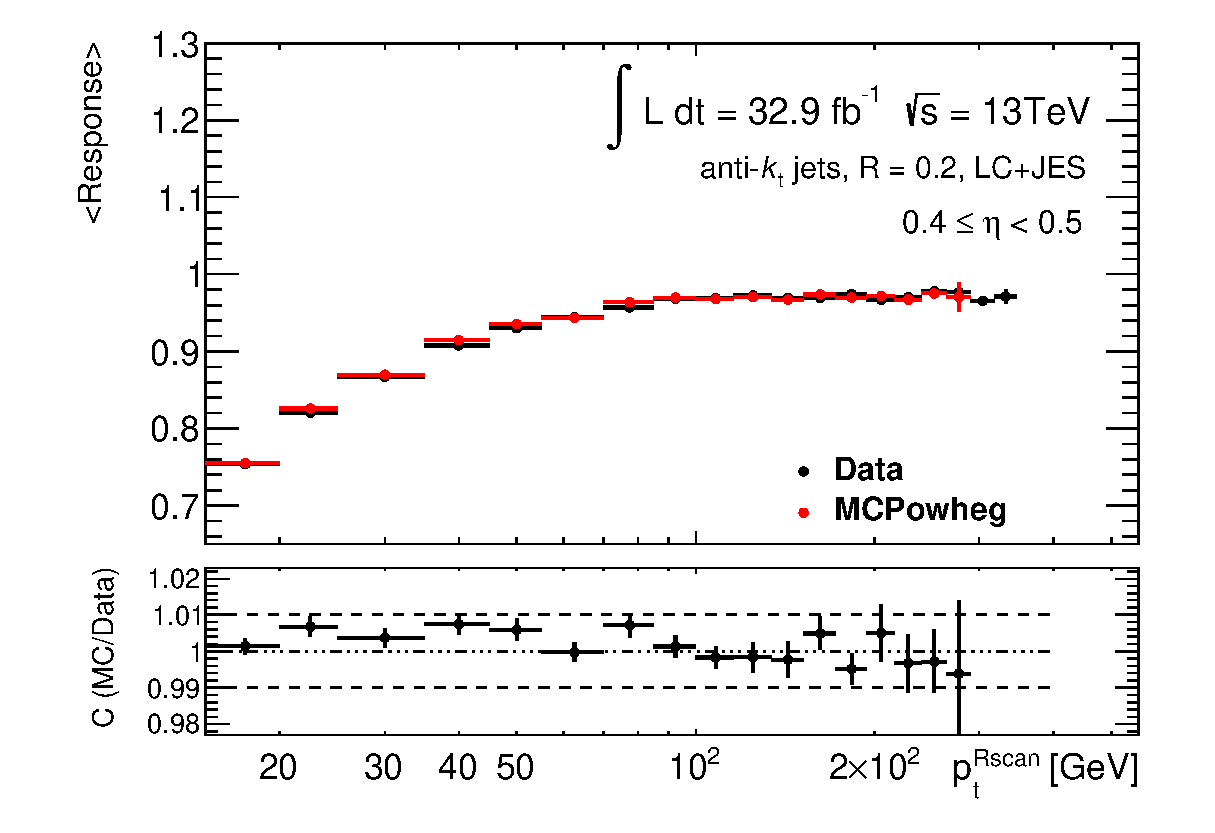
\includegraphics[width=\textwidth]{images/Closure2LC_49}
        \caption{$R=$0.2 ; 0.4$<\eta^{Rscan}_{det}<$0.5}
        %\label{fig:data2lc49}
    \end{subfigure}
    \hfill
    \begin{subfigure}[b]{0.495\textwidth}
        \centering
        \includegraphics[width=\textwidth]{images/Closure2LC_69}
        \caption{$R=$0.2 ; 2.4$<\eta^{Rscan}_{det}<$2.5}
        %\label{fig:Th26lc}
    \end{subfigure}
    \vfill
    \begin{subfigure}[b]{0.495\textwidth}
        \centering
        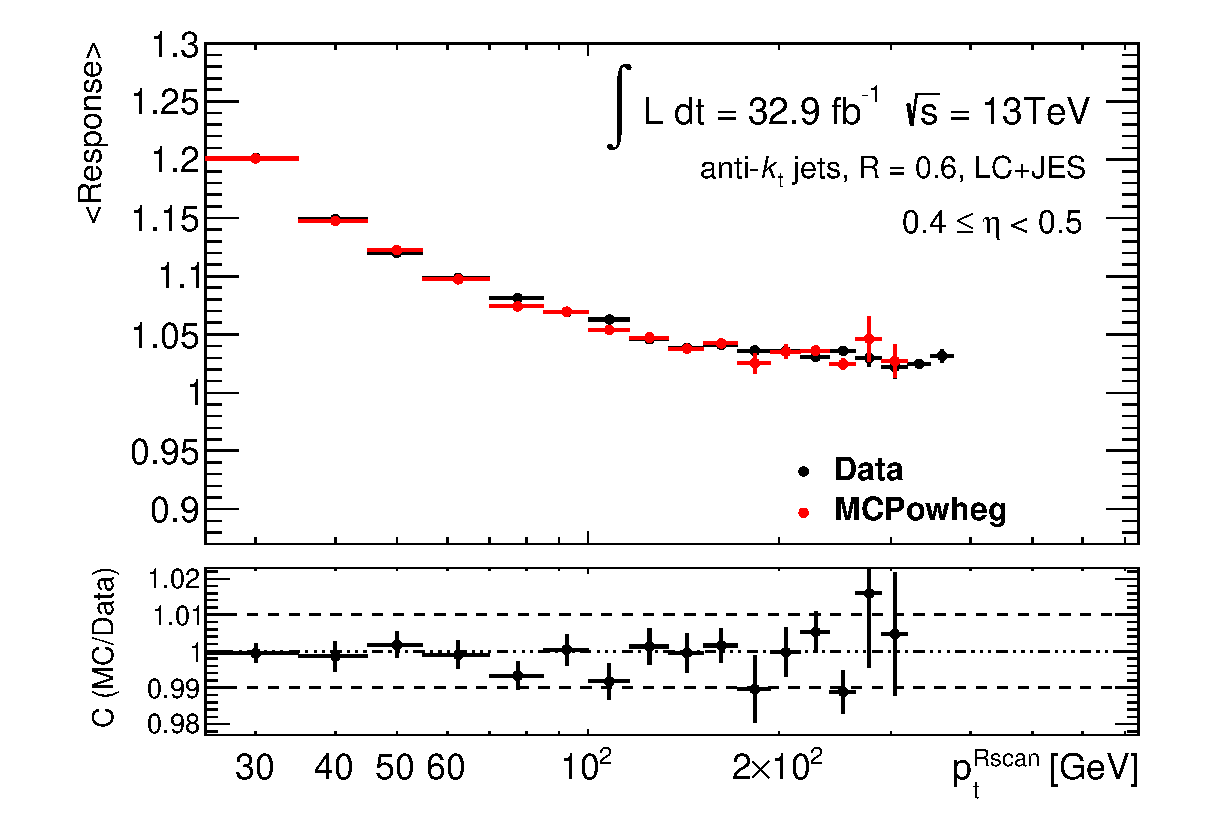
\includegraphics[width=\textwidth]{images/Closure6LC_49}
        \caption{$R=$0.6 ; 0.4$<\eta^{Rscan}_{det}<$0.5}
        %\label{fig:fitFeo}
    \end{subfigure}
    \hfill
    \begin{subfigure}[b]{0.495\textwidth}
        \centering
        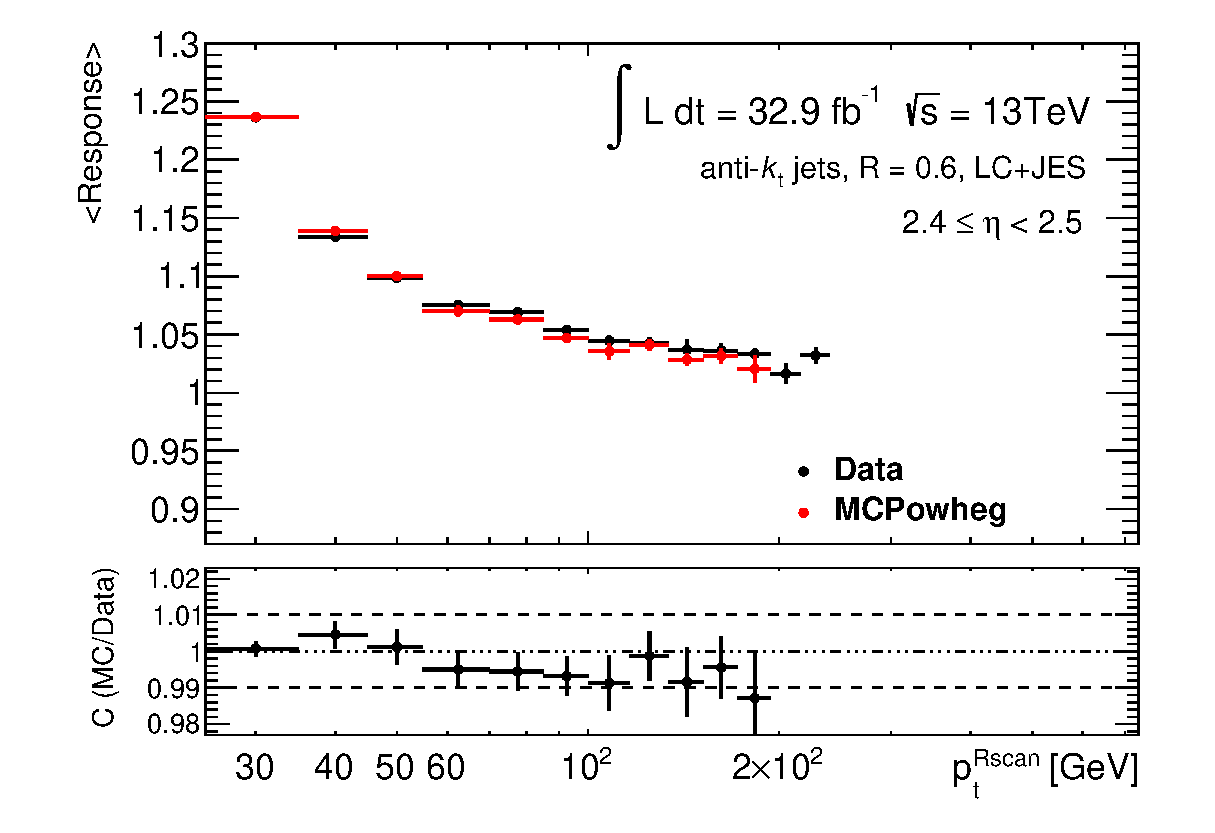
\includegraphics[width=\textwidth]{images/Closure6LC_69}
        \caption{$R=$0.6 ; 2.4$<\eta^{Rscan}_{det}<$2.5}
        %\label{fig:Th26lc}
    \end{subfigure}
    \caption{ En las figuras se muestra en rojo la response en la muestra nominal de MC, Powheg+Pythia, tal y como se construyó en la sección \ref{Derivandow}. En negro, se muestra la response de los datos construida ahora con Rscan Jets cuyo momento ha sido corregido por la calibración derivada en \ref{Derivandow}. En los paneles superiores se muestran $<\mathcal{R}>$, en función de $p_t^{Rscan}$, luego de atravesar el mismo proceso de selección de eventos y recortes cinemáticos que al derivarse la calibración. En los paneles inferiores se muestra el cociente entre $<\mathcal{R}>_{MC}$ y $<\mathcal{R}>_{Datos+InsituCorr}$. Las líneas punteadas representan la región de ancho de 2$\%$ de diferencia entre datos y MC.}
    \label{fig:Closure}
\end{figure}


%There are small deviations visible, but they are randomly distributed and they correspond to points with large uncertainties.